\documentclass[a4paper,12pt]{article}
\usepackage{amsmath}
%\usepackage{polish}
\usepackage[polish]{babel}
\usepackage[utf8]{inputenc}
\usepackage[T1]{fontenc}
\usepackage{graphicx}
\usepackage{anysize}
\usepackage{enumerate}
\usepackage{times}
\usepackage{plain}
\usepackage{caption}
\usepackage{graphicx}
\usepackage{setspace}
\usepackage{multirow}
\usepackage{lipsum}
\usepackage{listings}
\usepackage[colorlinks=true]{hyperref}
\usepackage[toc, nopostdot, nonumberlist]{glossaries}
\usepackage{indentfirst}
\hypersetup{
  colorlinks=true,
  linkcolor=blue,
  filecolor=magenta,
  urlcolor=cyan,
}
\urlstyle{same}
%\marginsize{left}{right}{top}{bottom}
\marginsize{2.5cm}{2.5cm}{2.5cm}{2.5cm}
\setlength{\parindent}{4em}
\setlength{\parskip}{1em}
\renewcommand{\baselinestretch}{2.0}

\lstset{basicstyle=\small\ttfamily,breaklines=true}
\lstset{framextopmargin=50pt,frame=bottomline}

\makeglossaries
\loadglsentries{glossaries}
\glsaddall

\begin{document}
\onehalfspacing
\begin{figure}[!htb]
  \centerline{
\includegraphics[scale=0.8]{images/agh_logo.jpg}}
\end{figure}

\begin{center}
  \Huge{Studio projektowe 1\\}
  \Large{Benchmark solverów prover9 oraz SPASS\\}
  \vspace{5cm}
  \Large{	Autorzy:\\
    Mateusz Grzeliński\\
  Przemysław Michałek\\}

  \newpage
\end{center}

\tableofcontents
\newpage

\section{Streszczenie}

Celem projektu jest zbadanie wydajności automatyczych metod dowodzenia twierdzeń Prover9 oraz SPASS. Na początku zostaje wygenerowna formuła \gls{SAT}, która zostaje rozwiązana przez badane provery. Badany jest czas wykonania, rezultat (czy SAT jest spełnialny), użycie pamięci RAM.
Generowana formuła SAT jest modufikowana ze względu na długość formuły, ilość zmiennych.

\section{Benchmark - strategia blackbox}

W stategii blackbox traktujemy provery jako czarny skrzynki - nie ingerujemy w wykonywany program, badamy tylko input oraz output. Dla każdego provera dostępne są:

\begin{itemize}
  \item czas wykonania
  \item użycie pamięci RAM
\end{itemize}

Zbadane zostaną statystyki proverów ze względu na następujące właściwości formuły SAT:

\begin{itemize}
  \item ilość zmiennych
  \item stosunek ilości formuł do ilości zmiennych
  \item czy formuła jest w postaci \gls{CNF}
\end{itemize}


\begin{figure}[!htb]
  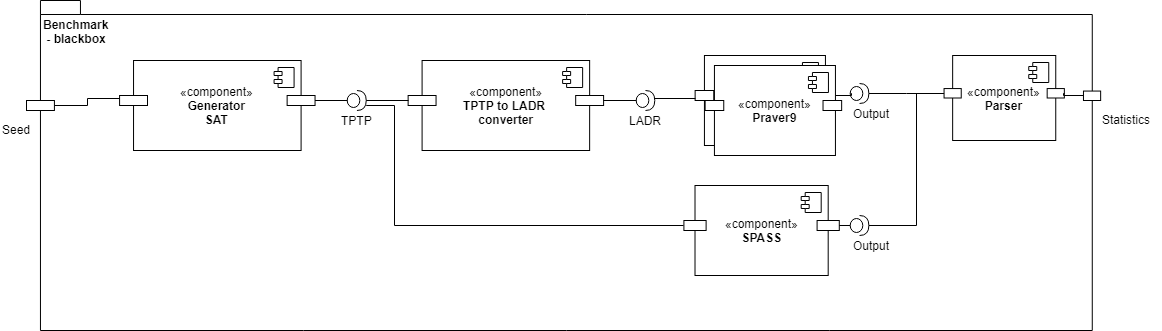
\includegraphics[scale=0.4]{images/studio-projektowe1.png}
  \caption{Diagram komponentów systemu benchmarka}
\end{figure}

\newpage

\subsection{Prover9}

Prover9 jest to zautomatyzowane narzędzie udowadniające dla logiki pierwszego rzędu stworzone przez Williama McCune’a.

Prover9 dostępny jest jako plik wykonywalny, przyjmuje pliki w formacie \gls{LADR}. Ilość opcji dostępnych z lini komend jest minimanlna, jedyną ważną opcją z punktu widzenia benchmarka jest
\lstinline{-x - set(auto2).  (enhanced auto mode)}

Oficjalna strona internetowa \url{https://www.cs.unm.edu/~mccune/mace4/}


\lstinputlisting[caption={Przykład pliku wejściowego w składni LADR}]{listings/prover9_example.in}
\lstinputlisting[caption={Przykład wyjścia Provera9}, basicstyle=\footnotesize\ttfamily]{listings/prover9_example.out}
\subsection{SPASS}

SPASS Theorem Prover jest narzędziem do automatycznego dowodzenia twierdzeń, należących do rachunku predykatów pierwszego rzędu.

SPASS nie korzysta z żadnych bibliotek, dostępny jest jako plik wykonywalny. Akceptuje pliki w składni TPTP lub swojej własnej. SPASS udostępnia wiele opcji z poziomu lini komend. Z punktu widzenia benchmarka istotnymi są:

\begin{itemize}
  \item TODO
\end{itemize}

\noindent
Wszystkie opcje linii komend \url{https://webspass.spass-prover.org/help/options.html}
\noindent \newline
Oficjana strona internetowa \url{https://webspass.spass-prover.org/}

\lstinputlisting[caption={Przykład pliku wejściowego w składni SPASS}]{listings/spass_example.in}
\lstinputlisting[caption={Przykład wyjścia SPASS}, basicstyle=\footnotesize\ttfamily]{listings/spass_example.out}

\subsection{TPTP}

TPTP - \textit{ ang. (Thousands of Problems for Theorem Provers)} - to biblioteka problemów wykorzystywanych do testowania systemów ATP. Jednocześnie jest to nazwa formatu, w którym zapisywane są te testy. TPTP udostępnia te problemy na oficjalnej stronie intenetowej.
Te problemy są sklasyfikowane przez domeny (3 literowe skróty), przykładowo
LCL - Logic Calculi,
COL - Combinatory Logic

\noindent
Oficjalna strona internetowa \url{http://www.tptp.org}
\newline
Pełny spis domen \url{http://www.tptp.org/cgi-bin/SeeTPTP?Category=Documents&File=THFSynopsis}
\newline
BNF składni TPTP \url{http://www.tptp.org/TPTP/SyntaxBNF.html}

\lstinputlisting[caption={Przykład pliku w składni TPTP}]{listings/tptp_example.p}

\subsection{TPTP to LADR}

W bibliotece \gls{LADR}, która jest załączona wraz ze źródłami Provera9, dostępny jest translator składni TPTP do LADR. Jest to plik wykonywalny.

\subsection{Parser}

Zadaniem parsera jest wydobycie dodatkowych informacji statystycznych o przebiegu działana proverów, na podstawie ich wyjścia.
\newline
Każdy prover podaje inne dane na wyjściu, dostępne statystyki podane są w tabeli poniżej.

\begin{table}[ht]
  \centering
  \caption{Dostępne statystyki dla różnych proverów}
  \begin{tabular}{ |c|c|c| }
    \hline
    Prover & SPASS & Prover9 \\
    \hline
    SAT spełnialny & dostępny & dostępny \\
    \hline
    TODO & & \\
    \hline
  \end{tabular}
\end{table}


\subsection{Generator SAT}

Plik wykonywalny, który generuje formuły logiczne w formacie TPTP. Funkcjonuje jako osobny projekt, dlatego został opisany w sekcji \ref{LFG}

\section{Generator formuł logicznych}\label{LFG}

Generator formuł logicznych - \textit{ang. LFG - Logic formula generator} - losowy generator formuł SAT

\subsection{Wejście}

\begin{itemize}
  \item seed - opcjonalnie - umożliwia powtarzanie losowania
  \item typ generatora liczb losowych
  \item ilość formuł
  \item ilość zmiennych
\end{itemize}

\subsection{Wyjście}

\begin{itemize}
  \item string w formacie TPTP (dokumenty do składni: http://www.tptp.org/)
\end{itemize}

\subsection{Algorytm}
\begin{itemize}
  \item Wypisz metadane jako komentarz (link do źródła, parametry wejściowe)
  \item TODO
\end{itemize}

\section{Wnioski}
\lipsum[1]

\printglossary


\end{document}
